
\section{INTRODUCTION} 
During the latest stage of structure formation, the universe gave birth to
non-linear, hierarchical structures known as galaxy clusters. 
These clusters, made up of dark matter, galaxies and hot gas,
are constantly accreting, merging and evolving with their
environments. Bright galaxies that belong to a galaxy cluster or group, in 
particular, highlight the overdensities of the underlying dark matter (DM) 
distribution. 

% Peaks, summary statistics 
% Modeling galaxy clusters - distributions, peaks, centroids 

In these dense regions of the clusters, the rates of particle
interactions can be enhanced, including the long-suspected self-interaction of DM
particles (hereafter, SIDM).  
Many papers have used the offsets between the summary statistics of the DM
density and the galaxy density to give constraints on 
the self-interaction cross
section, i.e. $\sigma_{\rm SIDM}$, of dark matter. 
A lot of observational studies focus on using merging galaxy clusters
as they assume the high collisional velocity should further increase the chance
of detecting the effects of SIDM.
By assuming galaxies being relatively collisionless $\sigma_{\rm gal} \approx 0$, 
any offset of the DM population from the galaxy provides $\sigma_{\rm SIDM}$ 
relative to $\sigma_{\rm gal}$. 
These observational studies include \cite{Markevitch2004} and \cite{Bradac2006b}  
reporting an offset of 25 kpc for the Bullet Cluster;  
\cite{Dawson2013} reporting an offset of 129 kpc and 47 kpc for the southern
and the northern subcluster respectively;
and \cite{Jee2015} reporting an offset of 190 kpc for MACSJ1752.
However, other studies using 129 X-ray selected relaxed galaxy clusters, 
such as \cite{George2012a} also report offsets of the same order of magnitude,
between $50 - 150$ kpc. 

On the other hand, there are many staged simulations of mergers of galaxy
clusters that focused on detecting the signal from
SIDM. They have consistently reported offset signals from SIDM simulations 
on par with statistical 
uncertainties. 
These simulations have raised questions about how strongly the galaxy-DM offsets 
can constrain the effects of SIDM.
These staged simulation have parametric prescriptions of the spatial 
distribution of galaxies 
(\citealt{Randall2008d}, \citealt{Kahlhoefer14}, \citealt{Markevitch2004}, 
\citealt{Robertson2016}), such as an NFW profile, 
and may not have realistic DM substructures that surround the clusters. 
Common to these staged simulation is the negligible galaxy-DM offset when assuming  
$\sigma_{\rm SIDM} = 0 {\rm~cm}^2 /$ g.
\cite{Randall2008d} found an offset of only 1.8 kpc in the staged
simulation with $\sigma_{\rm SIDM} = 0 {\rm~cm}^2 /$ g using $10^5$ 
galaxy particles that have identical distribution as the DM population at the
beginning of their simulations. 
Kim and Peter et al. (2016) and \cite{Kahlhoefer14} also show null offset 
throughout their staged simulation with $\sigma_{\rm SIDM} = 0 {\rm~cm}^2 /$ g.
It is likely that these idealistic simulation settings do not  
show the contribution of statistical and observational uncertainties to 
the galaxy-DM offsets. 
When \cite{Kahlhoefer14} simulated SIDM with both low-momentum-transfer self-interaction 
and rare self-interactions of DM with high momentum transfer, they found maximum 
offsets that are $< 30$ kpc for $\sigma_{\rm SIDM}$ as high as 1.6 cm$^2$ / g.
The reported offset from \cite{Randall2008d}
for $\sigma_{\rm SIDM} = 1.24 {\rm~cm}^2 /$ g is only 53.9 kpc. 
While [TODO] Kim and Peter et al. (2016) found a maximum offset $< 50$ kpc for 
$\sigma_{\rm SIDM} = 3 {\rm~cm}^2 /$ g,
and \cite{Robertson2016} also found a maximum offset $\lesssim 50$ kpc  
 from a simulation suite of the Bullet Cluster with $\sigma_{\rm SIDM} = 1 {\rm~cm}^2 /$ g.

It remains unclear how large the galaxy-DM offset should be 
without SIDM purely due to observational uncertainties and statistical noise. 
We therefore, perform mock observations of the galaxies clusters of the
Illustris simulation to characterize the intrinsic scatter of the offsets without SIDM.  
Simply put, we perform a hypothesis test with the galaxy-DM offsets in
the Illustris simulation directly corresponding to our null hypothesis
$\mathcal{H}_0$, with: 
\begin{equation}
\begin{cases}
	\text{the null hypothesis }\mathcal{H}_0: \text{Cold Dark Matter (CDM)} \\
	\text{the alternative hypothesis }\mathcal{H}_1: \text{Self-interacting Dark
	Matter (SIDM)} 
\end{cases}
\end{equation}

This is the first study to investigate if it is a feasible
idea to use the galaxy-DM offsets given the main constraints from observations,
namely, the projections and the dynamical states of the galaxy clusters. These
latent variables are confounding and can increase the variance of
the population summary statistics of the galaxy-DM offsets of galaxy clusters.  

This exercise is further complicated by the fact that there is no theoretical
foundation showing which observable would be the most sensitive to 
SIDM. In fact, \cite{Kahlhoefer14} have argued that SIDM does not cause
significant galaxy-DM offsets. We explore the ways of computing the smallest 
galaxy-DM offsets from the Illustris simulation data. 

A second utility of computing the galaxy-DM offset is to 
for computing the cluster-mass distribution using optical survey data.
Understanding the closest optical proxy of the DM peak will enable 
mass-estimation via the stacking of weak lensing signal. 

% Another aspect of this study to find out the precision
% to which we can find the galaxy-DM offsets.  
Popular choice for computing the offsets involves first inferring the summary
statistic of each of the DM and the galaxy population of a cluster before
taking a difference.
While there are well established procedure driven by lensing physics for 
inferring the DM spatial distribution, there is no standard procedure for
mapping the sparse member galaxy distribution. 
We quantify the bias and uncertainty associated with the one-point summary
statistic for summarizing the physical state of a galaxy cluster. 
% Commonly used one-point statistic for quantifying the galaxy population of a
% galaxy cluster include:
% 1) centroid and its variants with the data weighted by various mass proxies, 
% 2) luminosity peaks (\citealt{Robertson2016}, Dawson blah), 
% 3) galaxy number density peaks,
% 4) brightest cluster galaxy (BCG) etc.
% For each cluster, these quantities do not necessarily coincide, 
% especially when there is asymmetry in the spatial distribution of the galaxy 
% cluster components. 

% Offsets between different statistical measures of the galaxy and the DM
% population are not going to be zero.
% Miscentering ?! want to capture the dominant component of the cluster 
% You only have one center when there is only ONE component 

% What are the observational methods for summarizing dark matter distribution?
% Weak and strong lensing are the most reliable methods for mapping the dark 
% matter distribution in a galaxy cluster. 
% Common to all the methods are the estimation of the density peaks. 
% Uncertainties affect the conclusion for the computation the hypothesis test / parameter
% estimation
% Previous work on quantifying galaxy-DM offsets included  
% What centroids they have used
% 
% Physical motivation for using the galaxy density peak 
% Observation footprints 
% 
% Under the assumed Lambda Cold Dark Matter ($\Lambda$CDM) cosmology, it is unclear 
% that how large the offset $\Delta \vec{s}$ should be. 
% % Why use simulation data to study the populations? 
% Other complications for studying galaxy clusters arise from observation
% limitations. There is not a lot of information that can help constrain the  
% line-of-sight distance of different components of a cluster. 


% Goals of the paper
% With the advent of large-scale optical sky surveys, 
% the number of identified galaxy clusters is growing quickly. 
% Existing catalogs such as the Abell catalog also contain
% peaks inferred
% from the different peak finding methods and the DM peaks. 
% at least 4000 clusters with at least 30 members. 
% The future Large Synoptic Sky Survey alone will identify over a hundred thousand galaxy
% clusters (CITE) in optical wavelengths. 
% It is important to verify the uncertainties associated with common
% summary statistics for studying galaxy clusters. Considering the large quantity
% of data, methods with manual tuning will not scale well. The manual biases may
% also make it hard to obtain consistent statistics from the samples.

In this paper, we 
1) extract realistic observables from the Illustris simulation for
comparison with observations, 2) explore the pros and cons of the different statistic for 
summarizing {\it the member galaxy population} of a galaxy cluster, 3)	
give estimates for the offsets between the summary statistics of the galaxy  
population and the DM population under $\Lambda$CDM cosmology, which we call 
\begin{equation}
	\Delta \vec{s} \equiv \vec{s}_{\rm gal} - \vec{s}_{\rm DM}.
\end{equation}
where $\bf{s}_{gal}$ and $\bf{s}_{DM}$ are the two-dimensional (2D) spatial
locations of the summary statistic of the galaxy population, and the density
peak of DM respectively. This gives
an estimate of the baseline scatter of offsets without any SIDM. And finally we 
4) examine the properties of the clusters that give outliers in 
the offset distribution and 5) investigate the  
correlations between the 3-dimensional properties of a cluster and the projected 
observables such as $\Delta s$. 
\begin{figure*}
	\includegraphics[width=\linewidth]{fig1_mass_richness.eps}
	\caption{ {\bf Left figure:} Mass distribution of the group / cluster sized 
		DM halos for different halo selection schemes. Mass estimates obtained by the
		FoF algorithm are labeled as  M$_{\text{FoF}}$.
		Masses centered on the most bound particle within a radius those the 
		average density is 200 or 500 times the critical density of the universe are 
		labeled as M$_{200c}$ and M$_{500c}$ respectively. 
		% Huge discrepancies between the $M_{500c}$ and $M_{\rm FoF}$ of the clusters 
		% indicate the presence of spatially
		% separated substructures for the clusters (See Fig. 
		% \ref{fig:select_peak_visualization}). 
		{\bf Right figure:} 
		Mass-richness relationship of galaxy clusters and groups with 
		$M_{\rm FoF} > 10^{13} M_{\odot}$ assuming different cosmological redshifts
		of the observed clusters. 
\label{fig:mass_richness}}
\end{figure*}

% Basic setup 
The organization of this paper is as follows:
In section \ref{sec:illustris_sim}, we will describe the physical properties of 
the data of the Illustris
simulation (\citealt{Vogelsberger2014}, \citealt{Genel2014a}), 
and the selection criteria that we have employed to ensure that the
quantities that we examine resemble observables but without noise and
systematics from observations. 
Then in section \ref{sec:methods}, 
we explain the methods for computing various 
one-point statistics of the spatial distribution of galaxies how we prepare our dark
matter spatial data to resemble convergence maps. We show the statistical performance
of the different summary statistics before we show the main results
in section \ref{sec:results}. In the discussion in section \ref{sec:discussion}, 
we list the implications of our
results and compare it to other simulations and observations. We also 
show how one may make use of the population offset statistical distribution
from the Illustris data to construct a two-tail p-value test with 
a null hypothesis of $\sigma_{\rm SIDM} = 0$. 

	Our analysis makes use of the same flat Lambda Cold Dark Matter ($\Lambda$CDM) cosmology
as the Illustris simulation. The relevant cosmological parameters are
$\Omega_\Lambda = 0.7274, \Omega_m = 0.2726$, and $H_0 = 70.4$
km~s$^{-1}$~Mpc$^{-1}$.

\section{THE ILLUSTRIS SIMULATION DATA} 
\label{sec:illustris_sim}
The Illustris simulation contains some of the most
realistic, simulated galaxies to date, making it especially suitable for 
verifying the properties of galaxy clusters. We obtained our data from 
snapshot number 135 (cosmological $z=0$) of the Illustris-1 simulation. The Illustris-1
simulation has the highest particle resolution and has incorporated the most 
comprehensive baryonic physics among the different Illustris simulation suites. 
The sophisticated galaxy formation model in Illustris-1 
includes star formation rate, and stellar evolution due to
environmental effects of the intracluster medium, such as ram pressure stripping and
strangulation and feedback from Active Galactic Nuclei (AGN) etc. \citep{Genel2014a}.
The physics of stellar
evolution were solved using a moving mesh code {\bf \texttt{AREPO}} \citep{Springel2010}.
The observable properties of galaxies were statistically consistent
with the Sloan Digital Sky Survey (SDSS) data
\citep{Vogelsberger2014}. 

As the stellar population in Illustris were evolved from the initial condition,
these makes the spatial distribution of galaxies in  Illustris data more 
realistic than galaxies that are prescribed onto DM-only cosmological
simulation data such as those used in \cite{Harvey2013d}.  
Gravitational effects in Illustris-1 have provided realistic dynamics and
spatial distribution of subhalos. The simulated effects include
tidal stripping, dynamical friction and merging. 
Since the profile of the galaxies clusters were not
provided in symmetrical, parametric forms, we can study 
how asymmetry in the cluster profile affects the estimate of our summary 
statistic. This data allows us to examine cluster galaxies
in a realistic, yet noise-free way. The softening length of the DM particles is
1.4 kpc and those of the stellar particles is 
0.7 kpc, both in constant comoving units \citep{Genel2014a}.

The two sets of data catalogs in use are obtained through two types of halo
finders. The catalog that maps particles to the halo of a certain cluster was 
created by the {\bf \texttt{SUBFIND}} algorithm. The friends-of-friends (FoF) 
finder \citep{Davis1985} was further used to identify the affinity
of galaxy-sized halos to a galaxy-cluster. 
These galaxy-size halos are referred to as {\it subhalos} and 
they are the dark matter hosts of what we refer to as galaxies in Illustris-1. 
\cite{Vogelsberger2014a} also extracted the 
absolute magnitude of each subhalo in
the SDSS bands of $g, r, i, z$ as part of the {\bf
\texttt{SUBFIND}} catalog using stellar population synthesis models.

For our analyses, we make use of galaxy clusters / groups 
with at least 50 member galaxies that are above a reasonable observation limit, 
i.e. apparent $i \leq 24.4$ which is the limiting magnitude of the DEIMOS
spectrometer on the Keck telescope, when we assume a cosmological redshift of $z = 0.3$
in the $i$ band. 
This is because of the relatively large statistical uncertainty if we try
to analyze clusters with less than 50 member galaxies. 
As indicated by the right-hand panel of Fig. \ref{fig:mass_richness}, a total of 43 clusters have 
survived this magnitude cut. These simulated galaxy clusters (or groups) have 
masses ranging from $10^{13} M_\odot $ to $10^{14} M_\odot$.  

\begin{figure}
	\centering
	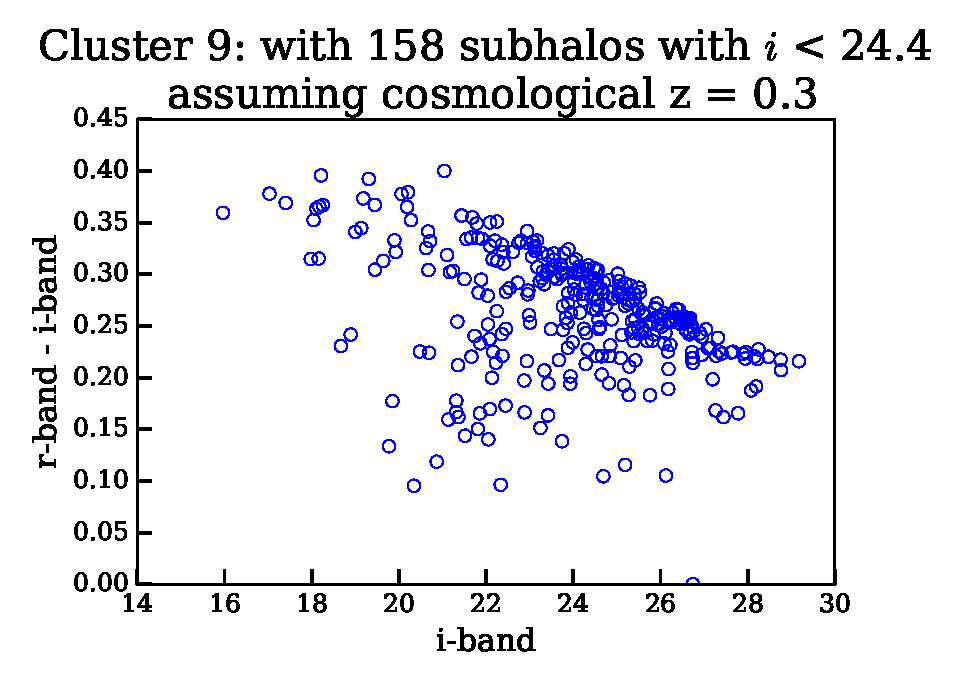
\includegraphics[width=\linewidth]{fig2_color_magnitude_diagram9.eps}
	\caption{Color-magnitude diagram of one of the galaxy clusters that is selected for 
		analysis. This cluster is the 9th most massive. 
		The apparent magnitude is calculated assuming that 
		the cosmological redshift (distance) is $z = 0.3$. 
		We can see a clear overdense region that corresponds to a red-sequence.
		The color-magnitude diagrams of the other clusters can be found in the
		Jupyter notebook at \href{https://github.com/karenyyng/galaxy_DM_offset/blob/master/code/analyses/fig2_color_magnitude_diagram.ipynb}{https://goo.gl/TJmI6s}.
		\label{fig:color_magnitude_diagram}
	} 
\end{figure}



% LSST goes as deep as 27.5

\subsection{Cluster properties}
\label{subsubsec:cluster_properties}

\subsubsection{Relaxedness of the galaxy clusters}

Clusters undergo merger activities of a large range of physical scales and 
in the time scale of million of years. 
The dynamical history, or what we call ``relaxedness" is hard to retrieve from 
simulations across different saved states and is missing from observations.
We quantify the state of the cluster by providing several quantitative
definitions of relaxedness and see how they correlate with $\Delta s$.
Some definitions of relaxedness referred by the simulation community
include:
\begin{itemize}
	\item the ratio of mass outside the dominant dark matter halo over the total mass
		of the galaxy cluster 
	\item the distance between the most bound particle from the center of mass as a
		function of $R_{200c}$.
\end{itemize}
which are computable from the Illustris data. 
To relate these simulation quantities, we compute more observation oriented 
quantities in the method section \ref{subsubsec:KDE}. 


\subsection{Selection of the field-of-view}
\label{sec:FOV}

\begin{table*}
\begin{center}
\begin{minipage}{180mm} 
	\caption{ Selection criteria for stellar subhalos (member galaxies) for each
		cluster / group 
\label{tab:member_galaxy_selections}} 
	\begin{tabular}{@{}lcccc@{}}
\hline 
Data &  Selection strategy  & Sensitivity & Relevant section  \\ \hline
Field of view (FOV) & FoF halo finder& comparable to FOV of the Subaru
Suprime camera & \ref{sec:FOV}  \\ 
Observed filter & $i$-band & consistent among the redder $r, i, z$ bands &   
\ref{subsec:galaxy_properties}
\\ 
Cluster richness  & $i \leq 24.4$ and $z = 0.3$  & sensitive to
the assumed cosmological redshift of cluster and & \ref{sec:illustris_sim} \\ 
& & the assumed limiting magnitude of telescope &   \\
Two-dimensional projections & even HEALPix samples over half a sphere &
discussed as results  & \ref{subsubsec:projections}\\  
\hline
\end{tabular} 
\label{tab:selection_criteria} 
\footnotesize{
}
\end{minipage}
\end{center} 
\end{table*}

We make use of the {\bf \texttt{SUBFIND}} member particle for the DM and the 
{\bf \texttt{FoF}} subhalo identification as our
default volume selection scheme for each cluster / group.
We understand that this choice of volume selection can be more ideal than
observational conditions. We make use of this volume selection scheme
for baseline comparisons. 

Assuming a conservative line-of-sight (los) distance 
, i.e. cosmological redshift, with [TODO] $z = 0.4$, 
the projected extent for most of the Illustris galaxy clusters and groups, 
fits inside the field of view of telescopes, such as the Subaru Suprime Camera,
which covers a physical area of [TODO] $\sim 9$ Mpc $\times 7$ Mpc. 
(See \href{https://goo.gl/ClZNvM}{https://goo.gl/ClZNvM} for a Jupyter notebook 
showing the extent of the Dark Matter distribution of the most massive 129 clusters)

\subsubsection{Spatial Projections}
\label{subsubsec:projections}
The summary statistics are computed all based on 2D projections of the
spatial location.
For computing the summary statistic, we note that 
the order of projecting the data and taking the summary statistic is
non-commutative.  
In order to represent the projection uncertainty, we compute even angular
orientation as our line-of-sight
by using HealPy, which is a Python wrapper for HEALPix\footnote{HEALPix is
currently hosted at http://healpix.sourceforge.net}
\citep{Gorski2005}. 
% The viewing angles of the projections are defined by an elevation angle
% $\xi$ and an azimuthal angle $\phi$. 
The number of projections that we employed is 384 for each cluster.
Details of the implementation of the projection is available in Appendix
\ref{app:projections}.

% \begin{table*}
% \begin{center}
% \begin{minipage}{180mm} 
% 	\caption{Comparison between various methods for estimating the one-point
% 		statistics of the galaxies of a cluster 
% \label{tab:centroid_comparison}} 
% 	\begin{tabular}{@{}lccccc@{}}
% \hline 
% Method &  One-point statistic & Sensitivity to biases & Uncertainty  & Relevant
% section & Comment  \\ \hline
% Centroid & 2D spatial averages & High & Low & \\
% Shrinking aperture & proxy for density peak & Higher sensitivity to substructures & Medium
% & \\
% Peak finding from KDE & density peak & Lower sensitivity to substructures &
% Higher & \\
% Brightest cluster galaxy & & Sensitive to foreground contaminants & \\ 
% Most bound particle & bottom of gravitational potential well &  & 
% &  \\
% \hline
% \end{tabular} 
% \label{tab:summary_stat_info} 
% \end{minipage}
% \end{center} 
% \end{table*}

\subsection{Properties of the galaxies in Illustris clusters}
\label{subsec:galaxy_properties}

Different galaxies have different masses, so they should not be considered with equal
importance for peak identification, which requires summing
the mass proxies of different galaxies. 
One of the most common weighting schemes employed for galaxy data is to weight
by the luminosity in a particular band. We make use of the $i-$band magnitude
associated with each subhalo as the weight. Since the $i-$band is
one of the redder bands, the mass-to-light ratio is not skewed as much due to star
formation activities. 
We further examined if the colors distribution of galaxies in Illustris-1 are
similar to the observed color-magnitude diagrams for clusters.
The Illustris cluster galaxies are realistic enough that it is easy to
identify an overdense region of galaxies known as the red-sequence in the 
color-magnitude diagram such as Fig.
\ref{fig:color_magnitude_diagram}. The red-sequence is prominent even if we
use other colors formed by different combinations of $r, i, z$ bands.

\section{METHODS}\label{sec:methods}
A common and the most precise way of summarizing the DM distribution in a
galaxy cluster is by finding the lensing peaks 
(\citealt{Medezinski2013}, \citealt{Markevitch2004}, \citealt{Zitrin13}).
Additionally, the peak region is physically 
interesting due to the higher particle density and interaction rates. 
The most direct analogous statistic for summarizing the member galaxy
population in a cluster is therefore, also the peak. 
Comparing the DM peak with the summary statistics of the galaxy population that
are not the peak therefore can have an {\it offset} purely due to the difference in
the choice of the statistic for summarizing the two sets of identically
distributed data. 
% Furthermore, galaxies are discrete. They are samples of the 
% There are many reasonable models for summarizing the overall spatial
% distribution of cluster components. Each method has different uncertainties.
% Our goal here is   
% not to identify galaxies as parts of subcluster components,
% but to find the location where we expect to see the highest mass density of the
% DM. We want to probe the region of the highest density. 
% Reasonable spatial models of cluster components 
% fall under several categories, 1) mixture models, 2) basis function
% expansions, such as wavelet methods \citep{Jauzac2014} and 3) non-parametric 
% density estimations such as a kernel density estimation, or 4) 
% hierarchical clustering methods such as DBSCAN. 
% Not only do the performance of the 
% first two methods depend heavily on model parameters such as the characteristic 
% scales of the basis functions or models, 
% the data fit also depend quite strongly on the functional form of 
% the underlying mixture model / wavelet basis. 
% While one can perform cross-validation to determine the charactistic scale for
% these methods, it is harder to automate the choice of the functional forms of the models.
% As we expect the signal due to SIDM is weak, it is desirable to use a model
% that is as precise and accurate as possible. 
% Often times,  the mixture models and wavelet bases 
% carry strong symmetry assumptions that may not be valid for spatial modeling of 
% hierarchically formed galaxy clusters that have more than one important physical 
% length scale. 
% This is because galaxy clusters have substructures over a wide range of length
% scales, from galaxy scales of hundreds of pc to fraction of a Mpc. 
% The symmetry assumption will bias the estimate of the point estimate that we
% are after for non-symmetric clusters.

% Goal: to identify the ``center'' of the light distribution. Here the adopted 
% tracers for the light distribution are the member galaxies of the cluster 
% and groups.

% We do not claim that point estimates are sufficient statistics for
% best representing the physical states of galaxy clusters nor the effect of
% SIDM. However, we try to understand the impact of the
% different choices of point estimates on the estimate of $\Delta s$. 
We compare four common point statistic or location for summarizing 
the member galaxy population in a galaxy cluster:
\begin{enumerate}
\item Weighted centroids
\item Weighted density peak via density estimate  
\item Shrinking aperture estimate
\item Brightest cluster galaxy (BCG)
\end{enumerate}

We avoid any manual methods for
comparison purposes, scalability and reproducibility. 
Since all the methods listed in this
paper are automated with the source code openly available, 
it is possible for future studies to reuse our code for comparisons. 
% There are a number of decisions ($\sim $[TODO] ADD NUMBER) that one needs to make to 
% determine the summary statistics. We will try to address the sensitivity of the offset
% due to each decision. 
Furthermore, a major advantage for automation is that it allows us  
to apply
the same methods across the different snapshots of the (Illustris) simulations to
examine the variability of $\Delta s$ across time. 


\subsubsection{Computing the weighted centroid}
\label{subsubsec:weighted_centroid}
We follow the usual definition of the weighted centroid is just: 
\begin{equation}
	\bar{\bf x}_w = \frac{\sum_i w_i \vec{x}_i}{\sum_i w_i},
\end{equation}
with $\vec{x}_i$ being the positional vector of each subhalo 
and we use the $i$-band luminosity 
as the weight $w_i$ for the $i$-th galaxy.
Centroids can be biased 1) by subcomponents from merging activities yet the
centroid estimate do not provide explicit evidence for ongoing merger or 
accretion. These estimates are also sensitive to odd boundaries 
of the field of view.

\subsubsection{Cross-validated Kernel Density Estimation (KDE) and the peak finder} 
\label{subsubsec:KDE}
Finding the exact peak of a sets of data points 
involves computing the density estimate of the data points and sorting through
the density estimates. A specific version of this density estimation process is
known as histogramming. During the making of histogram, each data point is
given some weight using a tophat kernel and the weights are summed up at
specific data locations (e.g. $\bf{x}_i$). 
Histogram is not good for peak estimate for {\it sparse} data for two reasons: 1) the
choice of laying down the bin boundaries strongly affects the count in each bin, 2) the choice of
bin width also strongly affects the count. Only when the available number of data points
for binning is large, the estimates of histograms and smoothed density
estimates are approximately the same. The number of member galaxies (< 500) 
is sparse enough for the uncertainty introduced by histogramming to bias our
peak estimate. For the density estimate of galaxy luminosity, 
we adopt a Gaussian kernel. 
The exact choice of the functional form of the smoothing kernel does
not dominate the density estimate as long as the chosen kernel is
smooth \citep{Feigelson2014}. 

The most important parameter of computing the density estimate is the bandwidth
 of the smoothing kernel, which takes the form of a matrix in the 2D case. 
 We illustrate the choice of kernel width with Fig.
\ref{fig:bias_variance_tradeoff}. When the kernel width is
too large (bottom left panel), the data is over-smoothed, 
resulting in a bias of the peak estimate. On the other hand, when the kernel
width is too small, it results in high variances of the estimate and result in
too many peaks due to noise. The decision of having to balance between creating high
bias or high variance estimates is also known as the bias-variance tradeoff. 

\begin{figure*}
	% \includegraphics[width=\linewidth]{figN_mass_richness.eps}
	\caption{This figure is adapted from \citealt{Vanderplas2012} from
\href{http://www.astroml.org/book\_figures/chapter6/fig\_hist\_to\_kernel.html}{http://www.astroml.org/book\_figures/chapter6/fig\_hist\_to\_kernel.html}
under the fair use of the BSD license. \label{fig:bias_variance_tradeoff}
}
\end{figure*}
A well-known way to minimize the fitting error from the density estimate is through
a data-based approach called cross-validation to obtain 
the optimal 2D smoothing
bandwidth matrix ($\Hmat$) of the 2D Gaussian kernel for the
density estimate $\hat{f}$:
\begin{align}
	\hat{f}(\chi; \Hmat) &= \frac{1}{n} \frac{1}{(2\pi)^{d/2}|\Hmat|^{1/2}}
	\sum_{i=1}^n w_i \exp((\chi-{\bf x}_i)^T H^{-1} (\chi-{\bf x}_i)),
	\label{eq:cross_validated_bandwidth}
\end{align}
where the dimensionality is $d=2$ for our projected quantities,
$\chi$ represents the uniform grid points for evaluation, and 
$\bf{x}_i$ contains the spatial coordinates for each of the identified member 
galaxies that survived our brightness cut and $w_i$ is again the $i-$band
luminosity weights for each galaxy.
The idea behind cross-validation is to leave a small fraction of data point 
out as the test set, and use the rest of the data points as 
the training set for computing the estimated density.
Then it is possible to minimize the asymptotic mean-integrated squared error
(AMISE)  by searching
for the best set of bandwidth matrix values, eliminating any free parameters. 

Specifically, we made use of the smoothed-cross validation \citep{Hall1992} 
bandwidth selector in the statistical package {\bf \texttt{ks}} \citep{Duong2007} 
in the {\bf \texttt{R}} statistical computing environment \citep{R_core}. 
Among all the different {\bf \texttt{R}} packages, {\bf \texttt{ks}} is the
only package capable of handling the magnitude weights of the data points 
while inferring the density estimates \citep{Deng2011}. 
Although the particular implementation of KDE has a computational runtime of $O(n^2)$, 
the number of cluster galaxies is
small enough for this method to finish quickly. 

After obtaining the KDE estimate, we employed both a first and second-order  
finite differencing algorithm to find the local maxima.  
The local maxima were then sorted according to the KDE density in a descending
fashion before we perform peak matching and compute the offset. The exact
procedure is discussed in section \ref{subsec:offsets}. 
% With the subdominant peak information, we investigate if the presence of subdominant peaks are correlated with
% $\Delta s$. 
% We provide scientifically accurate contours from the KDE 
% estimates from the cross-validated KDE method. 


\subsubsection{Shrinking aperture estimates}

Another popular method among astronomers for finding the peak of a spatial
distribution is what we call the shrinking aperture method.
While we do not endorse this method,
we test if the shrinking aperture method is able to reliably recover the 
densest peak.
This method is dependent on the initial diameter and the initial center 
location of the aperture.
This method does not evaluate if the cluster is made up of
several components.
The estimate using the shrinking aperture algorithm can be biased by
substructures. The only way to inform the algorithm about substructures would
be to introduce another parameter to restrict the center of the aperture, or to
partition the data with another (statistical) algorithm.
Furthermore, the convergence rate for this iterative algorithm is not
analytical and is dependent on both the data and the parameters. We use a
convergence criteria of having the aperture distance not change more than 2\% 
between successive iterations as a reference. The actual implementation in
Python can be found at \href{https://goo.gl/nqxJl8}{https://goo.gl/nqxJl8} while
the pseudo-code can be find in Appendix \ref{app:shrink_apert}.

\subsubsection{Brightest Cluster Galaxies (BCG)}
The BCGs are formed by the merger of many smaller
galaxies. The galaxy-cannibalism makes BCGs typically brighter than the rest of 
the cluster galaxy population by several orders of magnitude. 
However, star formation can cause
less massive galaxies to be brighter in the bluer photometric bands.
To avoid star formation from biasing our algorithm for identifying the
BCG, we find the brightest galaxies in redder bands i.e. the $r, i, z$
bands and found that they give consistent results for all selected clusters. 
We used the $i-$band to pick the BCG for the plots and the final results. 

\begin{figure*}
	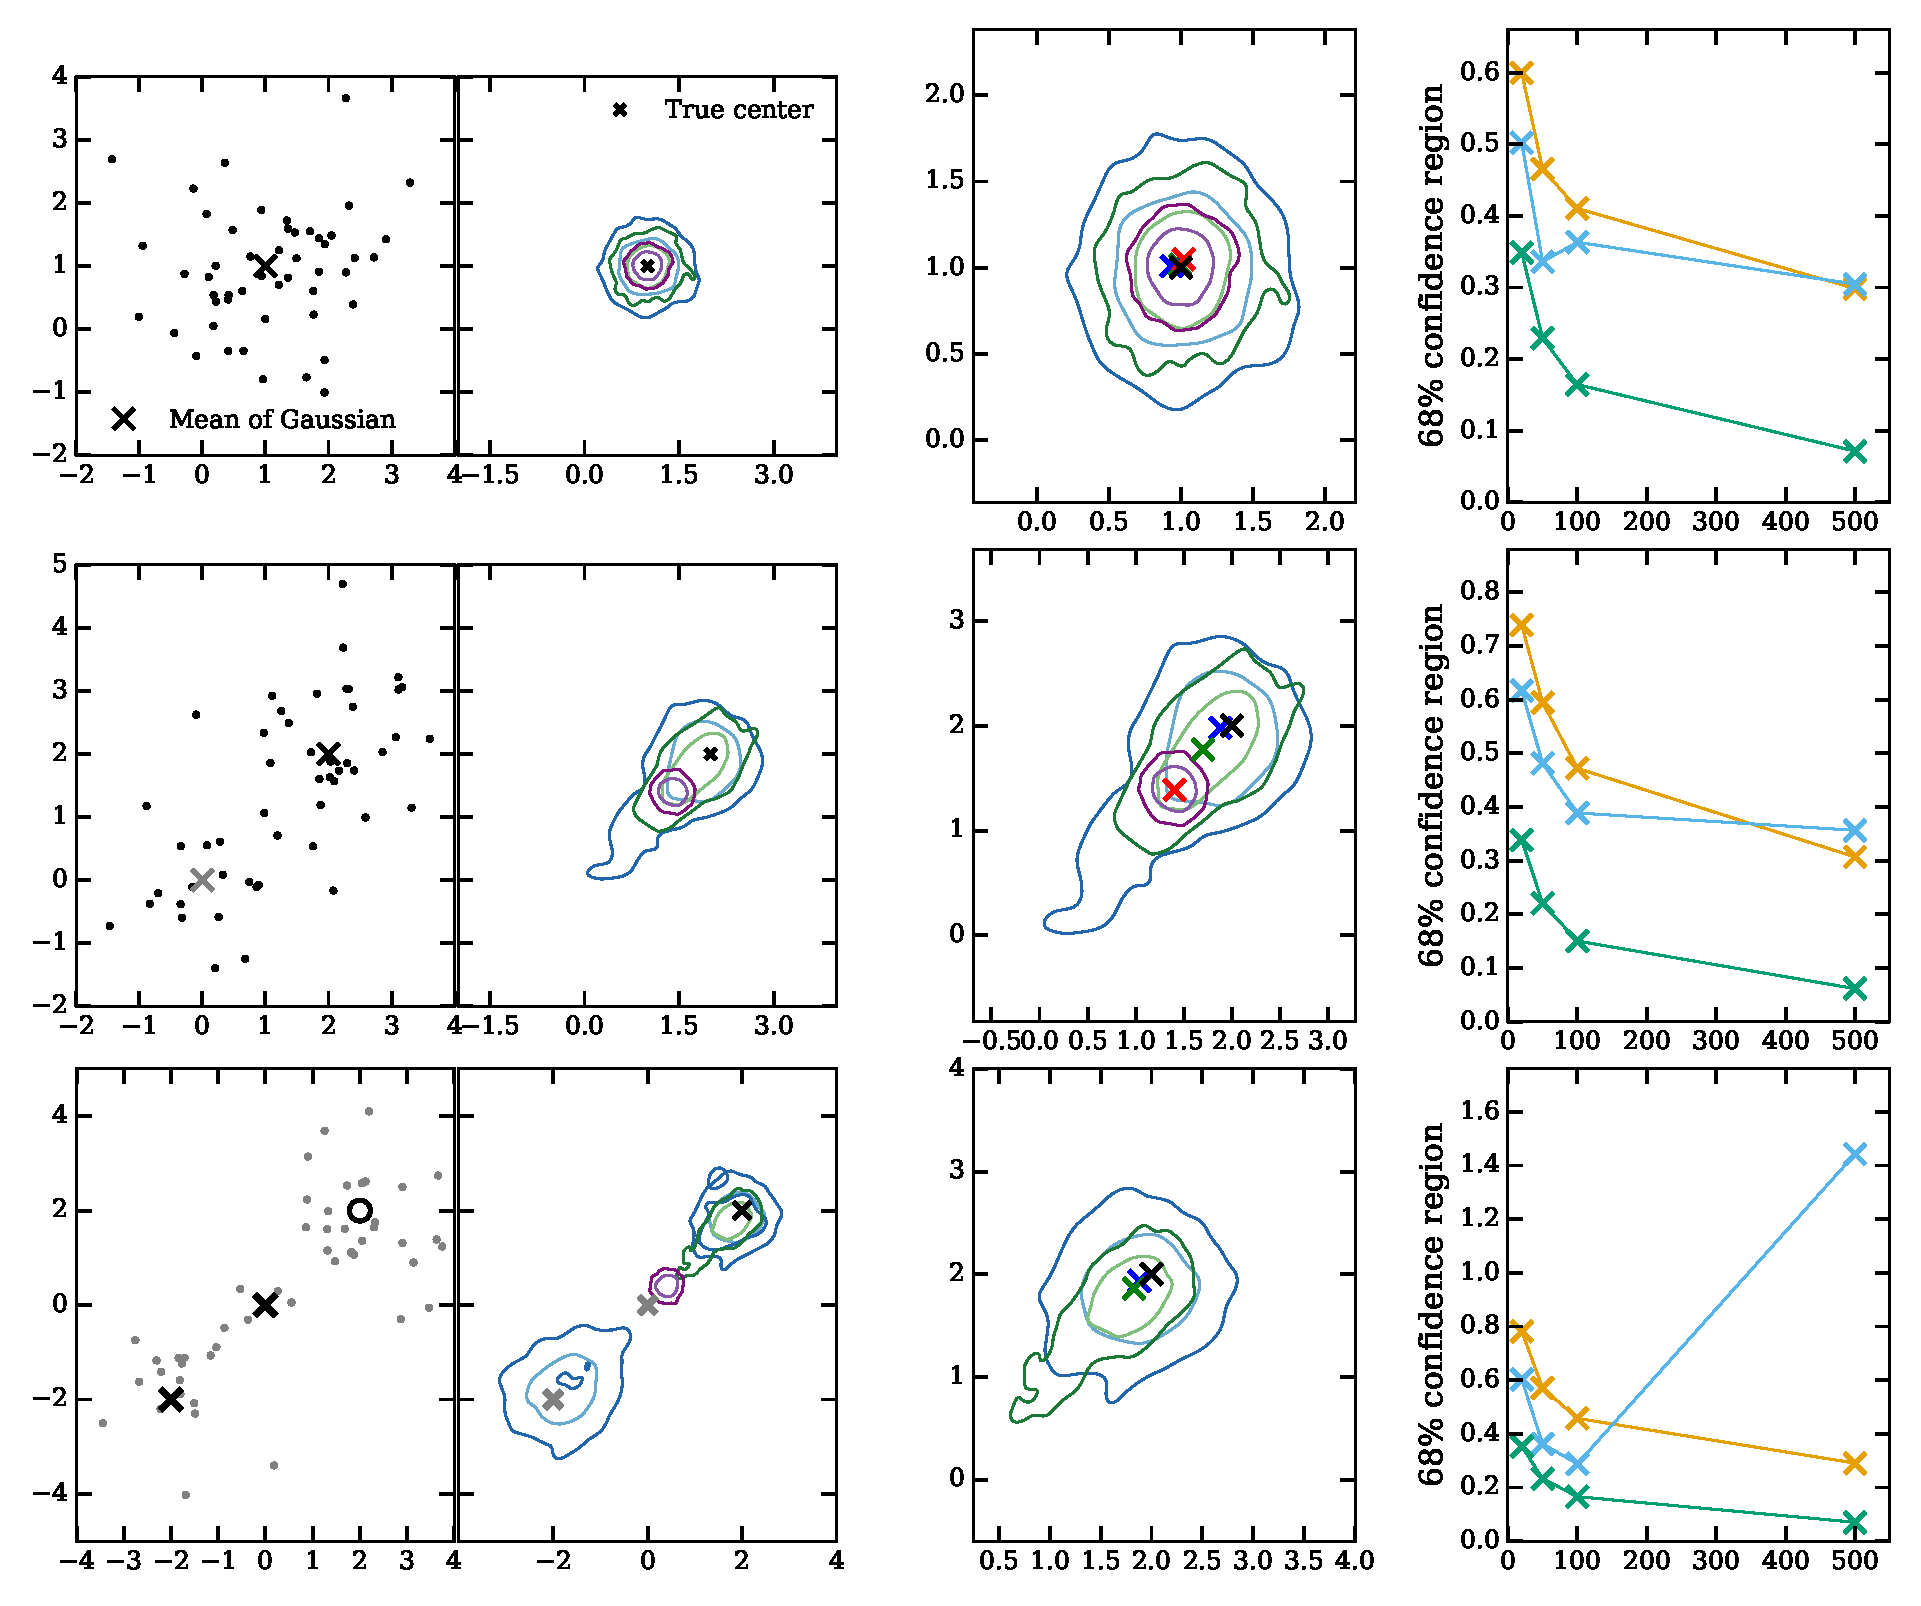
\includegraphics[width=.95\linewidth]{fig3_toy_data_mixtures.eps}
	\caption{Comparison of peak finding performances of different methods by
		drawing data points (i.e. 20, 50, 100, 500) from known number of 
		Gaussian mixtures. 
		Panels from the top row contain data drawn from a single Gaussian mixture. The
		panels from the middle row contain data from two 
		 Gaussian mixtures with weight ratio = 7:3. 
	The panels from the bottom row contain data drawn from three Gaussian
	mixtures with weight ratio = 55:35:10. 
	The left column shows how 50 data points drawn from the fixed number of 
	Gaussian mixtures look like. 
	Due to the statistical nature of this exercise, we sampled the data and
	performed the analyses [TODO: state how many times] many times to
	create the (68\% and 95\%) confidence contours of the estimates in the
	zoomed-in view of the data in the middle
	column. The rightmost column shows how the size (median contour radius) 
	of the confidence regions vary as a
	function of the number of drawn data points from the Gaussian mixtures. 
	From the middle and the rightmost
	column, we can tell that the KDE peak estimate is the most accurate but less
	precise for estimating the sampled data from each set of data. 
		\label{fig:toy_data_mixtures}}
\end{figure*}



\subsection{Comparison of the methods from Gaussian mixture data}
In order to examine the statistical properties of commonly used point-
estimates of the distribution of the galaxy data, we test them on data drawn 
from Gaussian mixtures with known mean and variance. (See Fig.
\ref{fig:toy_data_mixtures}). The main factors that affect the performance of 
the methods are sensitive to the statistical fluctuations of the drawn data, 
e.g. the
spatial distribution of the data, including 1) the density profile and 2) the
location(s) of subdominant mixtures,
, and 3) the number of data points that we draw.
It is also not enough to just
compare the performance by applying each method for one realization of the
data. We provide the 68\% and the 95\% confidence regions by applying the
each method for many Monte Carlo realizations.
In general, the peaks identified from the KDE density is closer to the 
peak of the dominant mixture (more accurate) than 
both the weighted centroid method and the shrinking aperture method.
For example, in the bottom middle panel, it is clear that the green contours
that represents the confidence region for the shrinking aperture peak is
biased due to the substructure, whereas the confidence region for the centroid 
is so biased that it is
outside the field of view of that panel.
For the bottom right plot, there is also a catastrophic outlier for the shrinking 
aperture method for 500 data
points. The outlier shows how the shrinking aperture method can have
radical behavior when there are subclusters in the data.	

\subsection{Modeling the DM map in Illustris-1 and the lensing kernel}
The most well established method of inferring the projected dark matter spatial 
distribution from observations is through gravitational lensing.
It works by detecting subtle image distortions of background galaxies due to
the foreground dark matter. The resolution of the inferred map therefore 
depends on the properties of the source galaxies that are being lensed, 
such as the projected number density, 
intrinsic ellipticities and morphology etc.
To achieve a sufficient signal-to-noise ratio for lensing, 
\citealt{Hoag2016}  has performed simulation for inferring the optimal size
for a Gaussian smoothing kernel for the cluster MACSJ0416. 
In the strong lensing regime, Hoag et al. found a resolution of 11 arcseconds
can best fit the data. This kernel translates to a physical size of 50 
kpc assuming a cosmological redshift of $z \approx 0.3$.
To compute a DM spatial distribution, we first make histogram with 2 kpc
$\times$ 2 kpc bin size which is larger than the DM softening length of 1.4 kpc. 
After that, we use a Gaussian smoothing kernel of the DM histogram Illustris DM
particle data. We do not perform a cross-validated KDE that has
$O(n^2)$ runtime on the DM data because the
number of DM particles for each cluster is of 
[TODO double check] the order of millions. The DM
resolution is high enough for the histograms to be accurate.  
Physically, the histograms of the dark matter of each cluster 
is analogous to a convergence map from a lensing analysis. 
% We show results after convolving the histograms with .   

% - [  ] Add the equation calculating a lensing kernel due to S/N constraint 
% apropos conversation with Marusa and Austin 's 



\subsection{Finding the offsets and its population distributions} 
\label{subsec:offsets}
It is possible to have several peak estimates from the KDE of the galaxy 
population. 
From the density estimate at each peak, we can sort 
the peaks according to their densities. We only match the peaks that are at 
least 20\% as dense as the densest galaxy-luminosity peak to avoid computing 
the offsets of negligible substructures, such as the peaks due to galaxies that
are located far away from the main concentraiton of mass.

In general, there are many more DM peaks because there are many more dark 
subhalos than galaxies for each cluster.  
To find the nearest match to the significant galaxy peaks,  
we construct a k-dimensional tree (KD-Tree) using the densest $n_{\rm DM}$ number of DM
peaks:
\begin{equation}
	n_{\rm DM} = \begin{cases}		
		3 \times (n_{gal} + 1) & {\rm if~} n_{gal} < 3 \\
	3 \times n_{gal}  & {\rm if~} n_{gal} \geq 3.
	\end{cases}
	\label{eq:peak_threshold}
\end{equation}
where $n_{gal}$ is the number of significant galaxy peak, and $n_{\rm DM}$
is the number of peaks that went into the construction of the KD-tree.
During the matching, we have $n_{\rm DM} > n_{\rm gal}$. When there are more
than one dense galaxy peaks located far away from one another, 
the top few densest DM peaks can be located around the same galaxy peak. 
i.e. there is no one-to-one matching between the luminosity of galaxies and the
density of detected DM peaks.
Matching purely based on density and luminosity leads to larger offsets.
From inspection, using eq. (\ref{eq:peak_threshold}) works well to match the appropriate
peaks. 

After matching the peaks, we aggregate the distribution of offsets for all the
clusters. The width of the marginal distribution 
$P(|\Delta s|)$ 
represents the uncertainty both from the different cluster masses, dynamical states
and the projections.
We provide the best estimated location of $P(|\Delta s|)$ using the biweight 
statistic \citep{Beers90}. 
Note that for 
\begin{equation}
	\Delta s = \sqrt{(\Delta x)^2 + (\Delta y)^2},
	\label{eq:var_transformation_caveats}
\end{equation}
where $\Delta x$ and $\Delta y$ are the two projected spatial offsets by
subtracting the DM peak coordinates from the galaxy peak coordinates.
We discuss the possible loss of information and the caveats of 
the variable transformation in eq. 
(\ref{eq:var_transformation_caveats}).
The biweight estimate will not center on zero even if $\Delta $





[TODO] make sure that the plots reflect this.

[TODO] talk about how I computed the offset / offset distribution for the KDE
peaks 

The inference of the estimated value and the confidence intervals will be 
incorrect after taking the absolute value of the offsets.
The projected offsets for different clusters and projections give us as
estimate of the population distribution of the offsets.


[TODO] talk about how I computed the other offsets, BCG / centroid /
shrinking aperture etc.

\section{RESULTS} 
\label{sec:results}

We summarize the main results here and leave the detailed tables of results in 
Appendix \ref{app:table_of_results}.


\begin{figure*}
	\begin{center}
	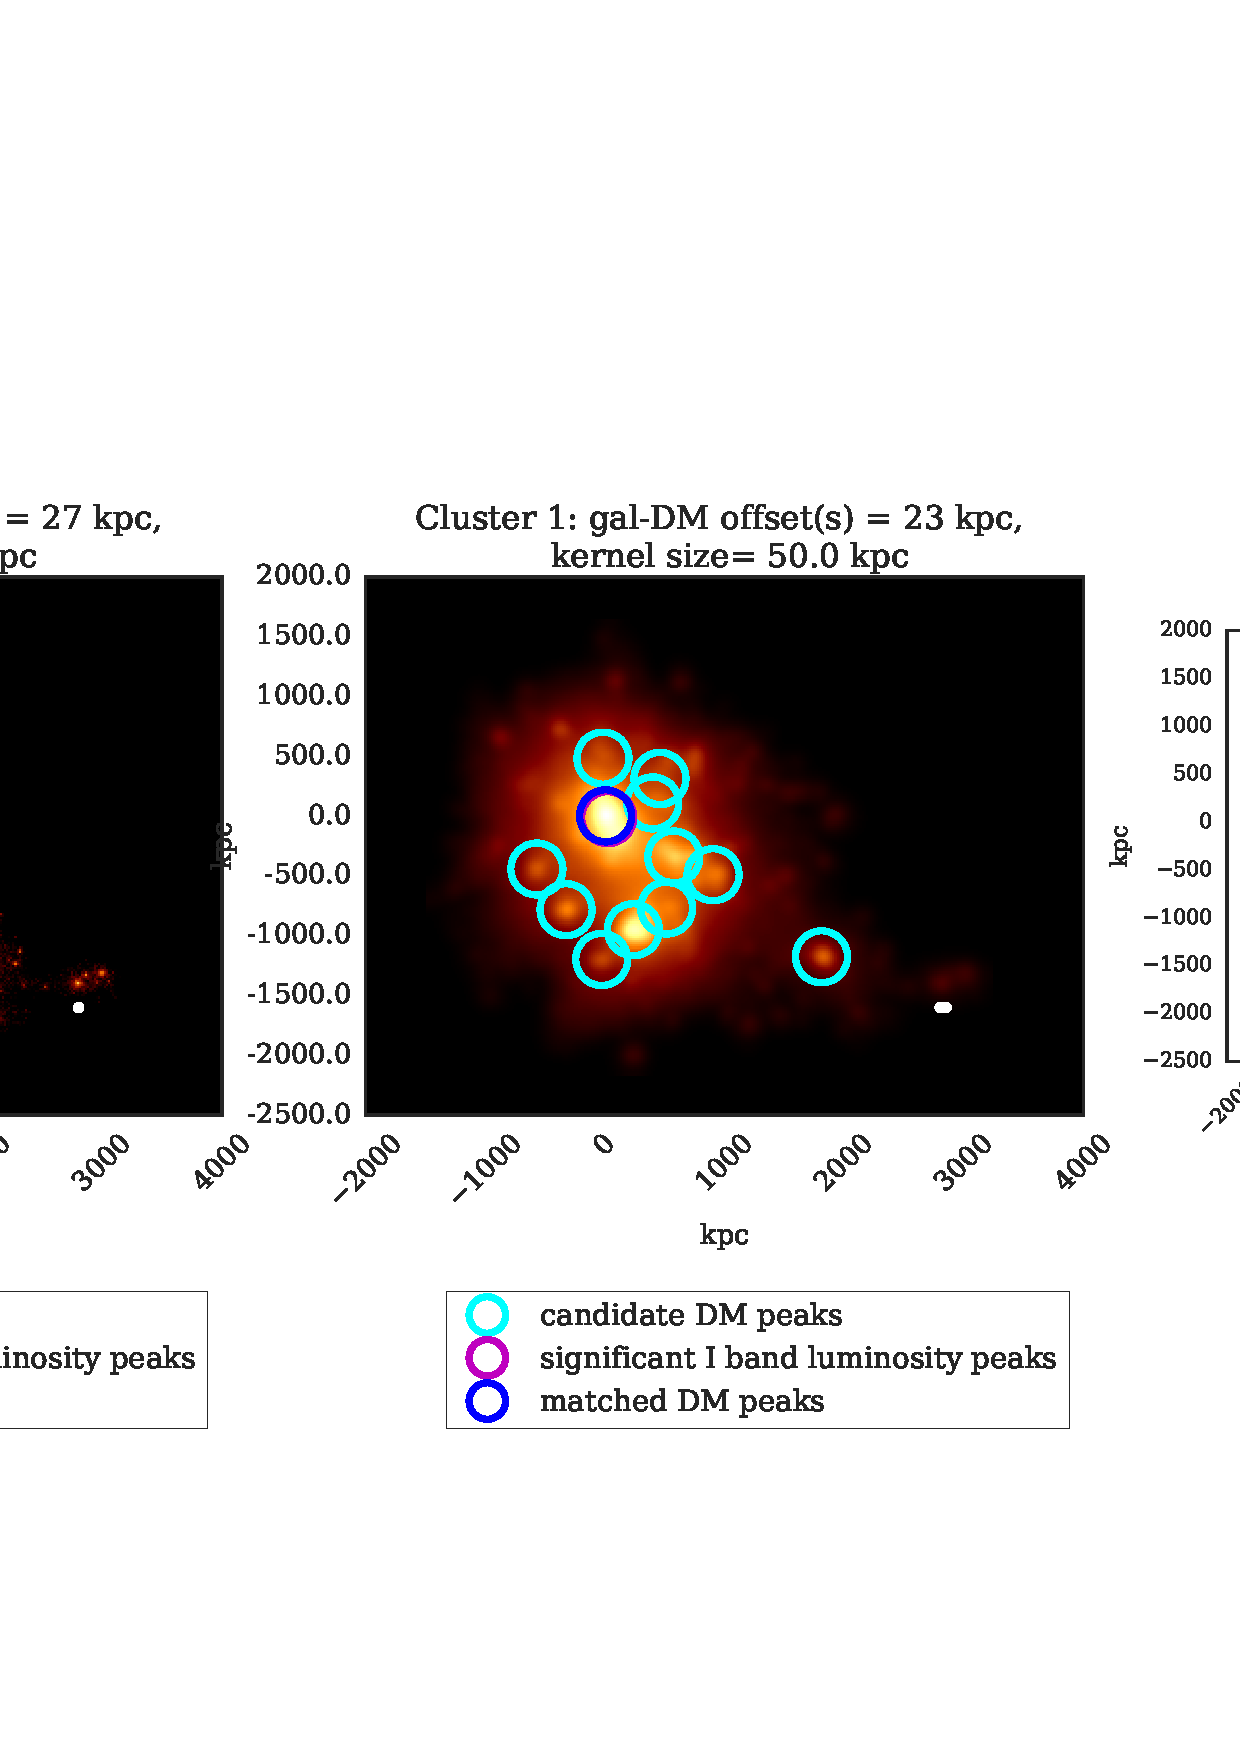
\includegraphics[width=0.85\linewidth]{Fig4_clst1_48_225.png}
	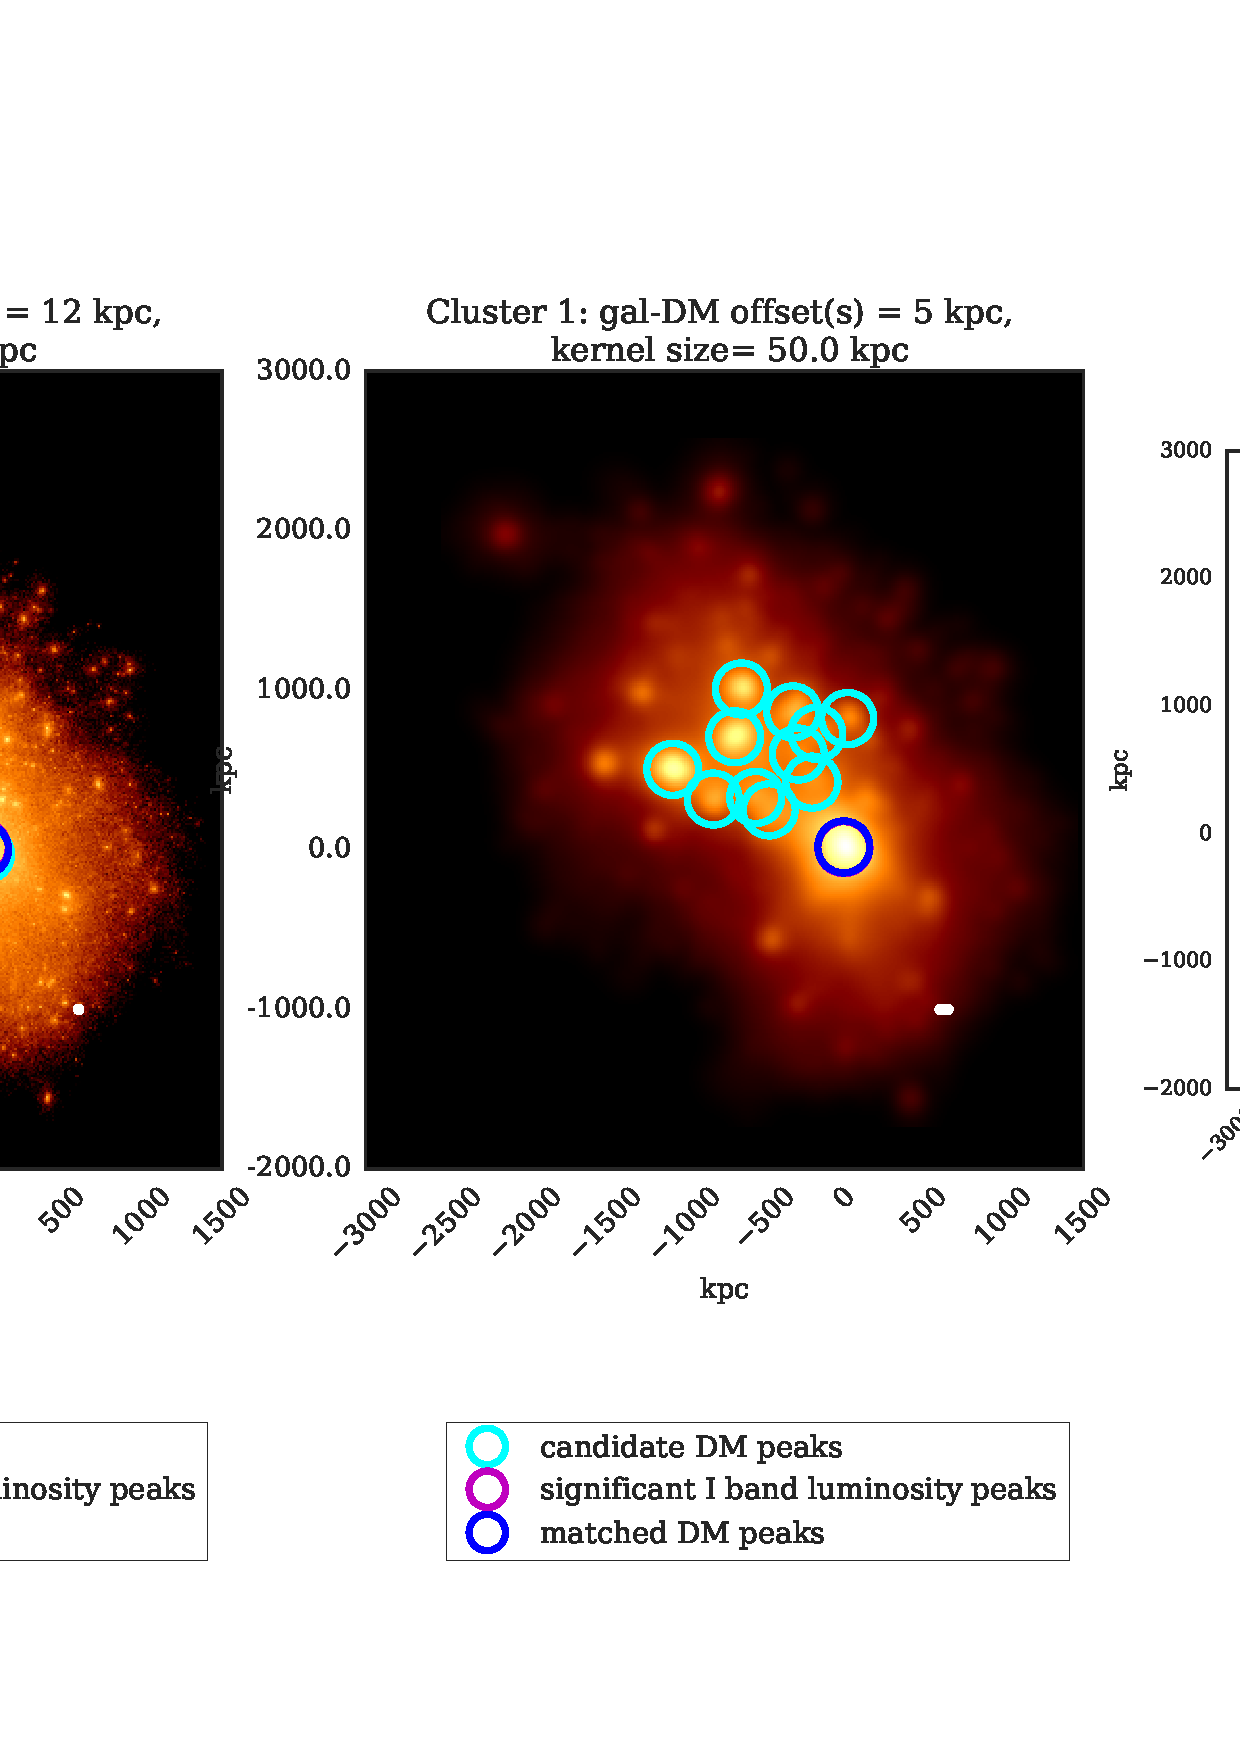
\includegraphics[width=0.85\linewidth]{Fig4_clst1_48_135.png}
	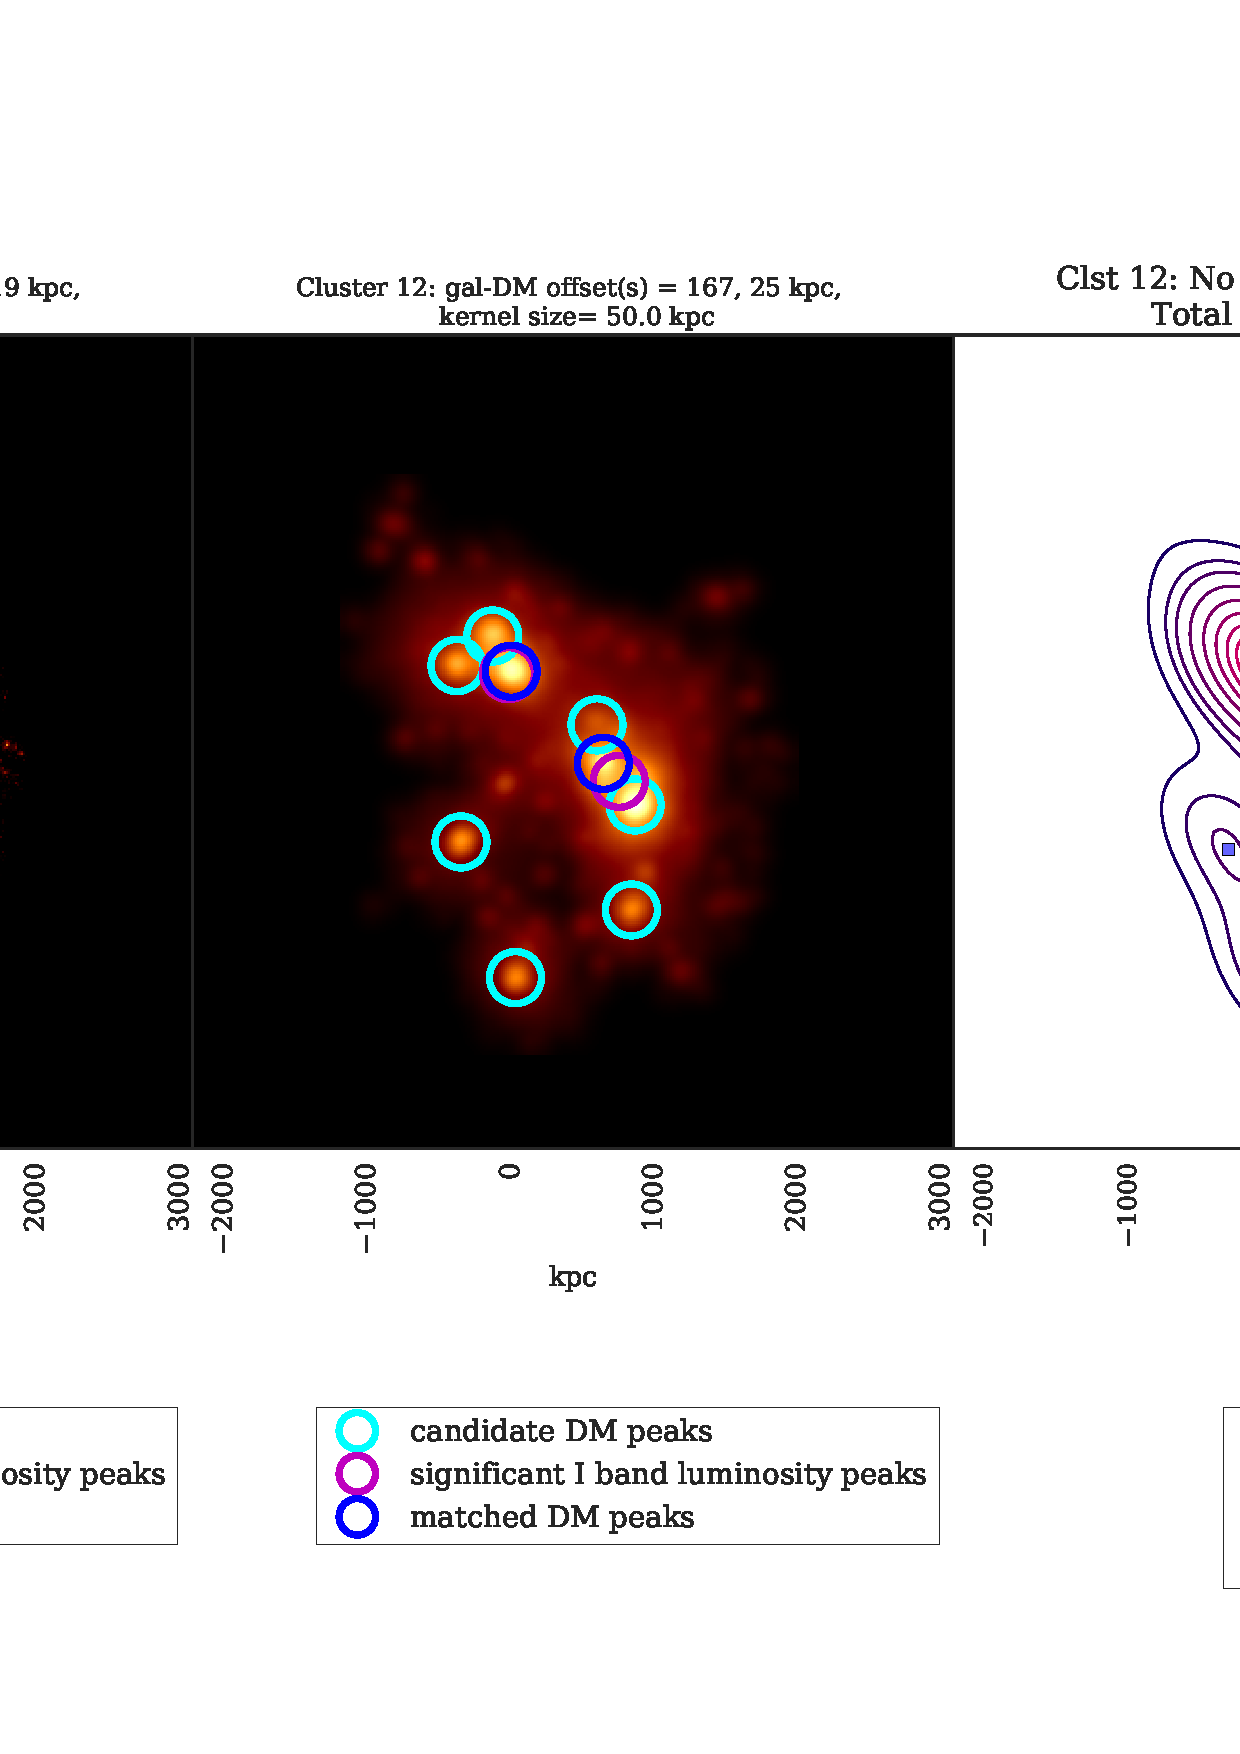
\includegraphics[width=0.85\linewidth]{Fig4_clst12_48_135.png}
	\caption{[TODO merge margin between left and middle panels] 
		Visualization of clusters (each row is for the same projection
		of the same cluster). {\bf Left column:} Projected density distribution of DM	
		particle data (density overlay). 
		The identified density peaks are indicated by colored circles. 
		{\bf Middle column:} The same DM projection but with treated with a 50 
		kpc smoothing kernel (kernel size indicated by white dot on lower right of
		the figure. Note that the thickness of the dot may be larger than 2 kpc
		for the plots on left hand column).
		{\bf Right column:} Projected galaxy kernel density estimates (KDE) of 
		the $i$-band luminosity map for the member
		galaxies of the same clusters. Each colored contour denotes a 10\% drop 
		in density mass starting from the highest level in red. Each of 
		the magenta ellipse on the
		bottom right corner of each plot show the Gaussian kernel matrix 
		$H$ from eq. (\ref{eq:cross_validated_bandwidth}). 
		The big black 
		circle is centered on the most bound particle as identified by {\bf
		\texttt{SUBFIND}} and the radius of the circle indicates the 
		three-dimensional region in
		which the average density is 200 times the critical density of the universe
		(a.k.a. R$_{\rm 200C}$).
		See \href{http://goo.gl/WiDijQ}{http://goo.gl/WiDijQ} 
		and \href{http://goo.gl/89edcM}{http://goo.gl/89edcM} for the 
		visualization of the selected clusters inside two Jupyter notebooks.
		\label{fig:select_peak_visualization}
	}
\end{center}
\end{figure*}


\subsection{Galaxy-DM Offset in Illustris}
% talks about the overview of the offsets in the simulation

\subsubsection{Two-dimensional(2D) offsets}
\begin{figure*}
	\begin{center}
	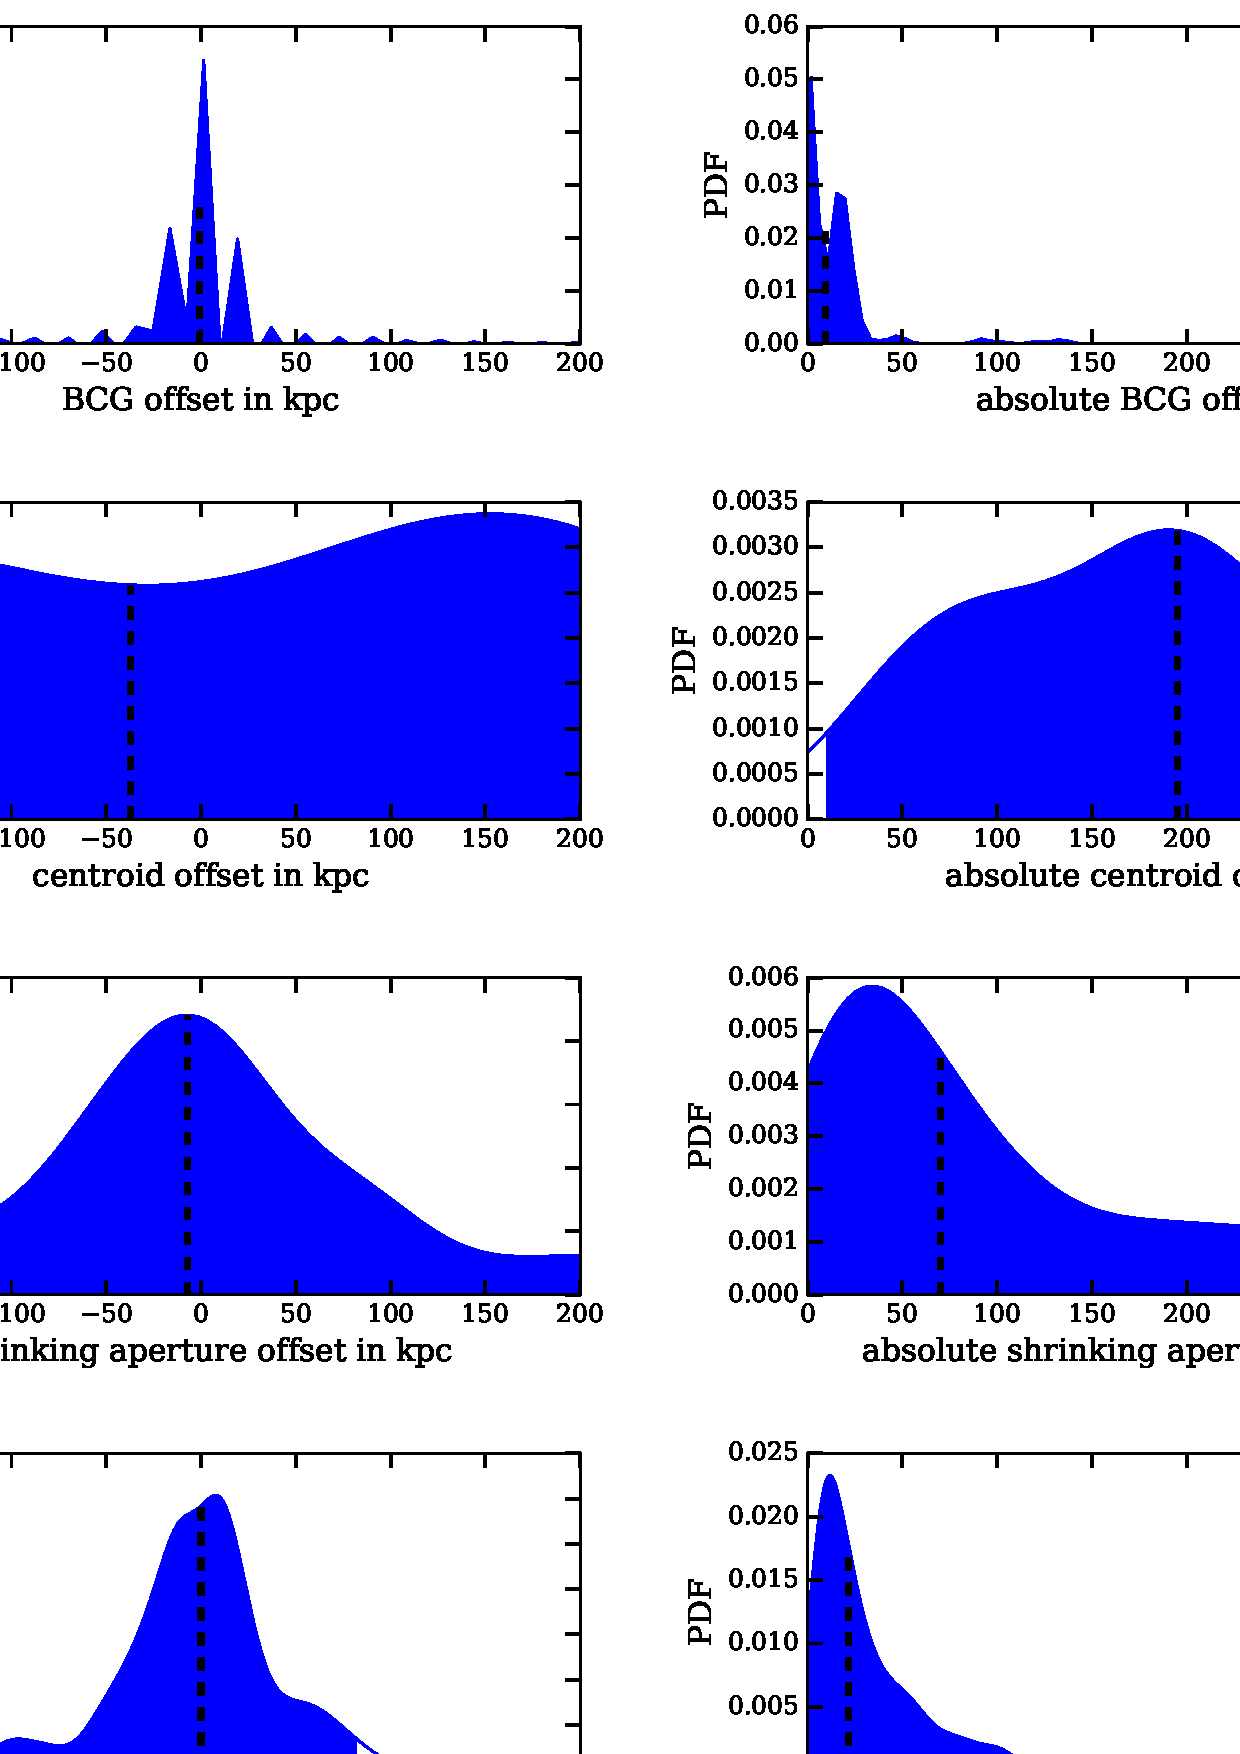
\includegraphics[width=0.65\linewidth]{Fig5_offset_distribution.png}
	\caption{ 		
		The distribution of different offsets of [TODO] clusters with [TODO]
		projections. The dark blue area indicates the 68\% confidence interval
		while the light blue area shows the 95\% confidence interval. 
		% We provide two ways of summarizing the offsets, the {\bf left column} shows
		% the offsets when we randomly denote the sign of the offset. The
		% direction of the offset in the Illustris simulation without SIDM has no 
		% physical meaning.
		% The estimates of the offsets on the left are all consistent with 0 within
		% the 68\% confidence interval.
		We plot the offset after taking the
		absolute magnitude, which  
		The estimates from the absolute magnitude of the
		offsets are pushed towards larger values. 				
		\label{fig:offset_distributions}
	}
\end{center}
\end{figure*}

From Fig. \ref{fig:offset_distributions}, we can tell that the population 
estimates. 

The variance of the offsets due to projection is [TODO].
In particular for the most massive galaxy clusters with $10^{14} M_{\odot}$



\begin{itemize}
\item those between BCG, the most bound particle and the other masses. 
\item explain the variation of the offsets for the same cluster under different 
projections 
\end{itemize}

While there is a tight distribution for $\Delta s_{\rm BCG}$ that peaks around
zero, there is a non-negligible population of data points that lies outside
this peak. 
[TODO] investigate what is WRONG with those outliers.

\subsection{Correlations between different variables and the offsets}
We subset the data and visually inspected the samples with the largest 
galaxy-DM offsets $\Delta s_{\rm KDE}$. We found that ...  

\subsubsection{Correlations between the offsets and properties of the 
cluster / groups}
[TODO] examine the relationship between
\begin{itemize}
\item 3D relaxedness
\item mass 
\item richness  
\end{itemize}



\section{DISCUSSION}\label{sec:discussion}
[TODO ]Density estimate based only on galaxy number density without luminosity 
weights do not resemble the DM distribution.


It is not easy to compare the result of this study to other study due to the 
differences in the multi-step method for inferring the ``peak", or the
"centroid".

\subsection{Other findings from the visual inspection of the simulated galaxy clusters}
From the high resolution visualization of the DM maps (two-dimensional
histograms with 2 kpc bins) in 
Fig. \ref{fig:select_peak_visualization}, we can tell that some clusters clearly
possess multiple subclusters with visible separations between the subclusters, 
e.g. cluster 12 visualized on the panels on row 3 of the plot. 
However, there are also many clusters that contain  
only one main component but show several closely-located density peaks in the
densest region. This illustrates why finding a `center' or peak of a cluster 
is an ill-defined notion. Most of the density-based statistics 
are only unambiguous for smooth, symmetrical data.  

Furthermore, we show a lower-resolution visualization of the DM surface
map in Fig. [TODO] compared to the higher resolution map, we can see a clear
shift in the peak location. This illustrates that peak / center finding is also
subject to noise from the data.

Sometimes when the peaks are mismatched, it is due to a resolution difference 
between the higher resolution DM data and the sparse galaxy data. 
(See middle bottom panel in Fig. \ref{fig:select_peak_visualization})



The main reasons for the existence of several peak estimates include:
1) Extended substructures that exist within the cluster, which we call
subclusters, although the boundaries of subclusters are ill-defined.
2) Galaxies that are located further away from the main concentration of mass.
These peaks are excluded based on density cuts.
3) This last case illustrates the difficulty of pinpointing a point-estimate
such as a `center` . It is 
possible to have more than one bright galaxies spatially close to the main
concentration of mass. 
(See the right most panel of Fig. \ref{fig:select_peak_visualization}
where the galaxy luminosity peaks are represented with squared markers that are
colored according to the relative density to the densest galaxy peak of that 
projection). 

\subsection{The statistical performance of different peak finding methods}
The difficulty in matching is not necessarily due to wrong algorithms.
When the substructures of several important physical scales are present due to
hierarchical clustering, peak finding is not a well defined problem.
It is possible for a smaller group-sized halo to be embedded in a
galaxy-cluster size halo, or several group-sized halo have the majority of its
mass overlapped with another halo.
There is no unique solution for specifying the physical boundaries of substructures
before finding the corresponding peaks. 
While the peak-matching by galaxy-peaks that
we performed is an ad-hoc approach, only picking spherically-looking can only
guarantee relaxedness up to a certain extent. 
The number of non-relaxed clusters far outnumber the ones that are dynamically 
relaxed. 

The situation is subsection{Comparison to other simulations}
\subsubsection{Comparison to other cosmological simulations}



Assume dynamical equillibrium 


\cite{Cui2015} X-ray center, BCG

does not provide the pairwise offset between the DM and the galaxy distributions
but rather the offset between the minimum potential and DM. 
computing the offset from the population statistic of the DM spatial distribution 
with the population galaxy distribution destroys the possible correlations.

Fig. 3 in \cite{Cui2015} shows both the DM peak and the galaxy offsets to the 
minimum gravity potential center but that representation destroys the 
correlations. 

kernel smoothing approach
use minimum potential position as a proxy for the maximum SPH density 

Voronoi Tessellation Density (VTD)

gives no confidence estimate for comparison. 
width of histograms can affect the distribution  
taking the absolute magnitude of the offset can bias the data  
\cite{Harvey2013d} consistent with zero offsets using the {\bf
\texttt{Wavedetect}} wavelet analysis algorithm. 
Galaxies prescribed to the DM simulation and not simulated to see 
how the surrounding environment  


Provided nice theoretical motivation for describing how galaxies and DM
population would behave 
They have only verified that their model of SIDM work for 
$\sigma_{\rm SIDM} = 0$ but not any model with $\sigma_{\rm SIDM} > 0$

\subsubsection{Comparison to other staged simulations}

In this work, we test purely for the offset due to statistical noise and
missing variables such as projection and impact parameter 

\cite{Randall2008d} can be thought of a controlled experiment where 
only the effects of SIDM is in place.
This is because a large number of tracer galaxies were painted on as 
collisionless particles, using identical distributions between the galaxies 
and the DM particles at the beginning of each run. 

Statistical uncertainties overwhelm the signal of SIDM.

\cite{Robertson2016}


[TODO] cite Stacey

The 

It is not clear about the ability of $\Delta s_{\rm SIDM}$ for differentiating 
between different $\sigma_{\rm SIDM}$ models. 

It is unclear that $\Delta s$ is a sensitive observable to signatures of
$SIDM$.


At $\sigma_{\rm SIDM} \approx 1.25 $cm$^2$ / g, 
\citealt{Randall2008d}, \citealt{Robertson2016} only found an offset of $50
kpc$, this is completely within the population uncertainties of offsets, 
while the projection uncertainty of a cluster can be as large as  
[TODO]$ $ kpc.


Bullet cluster 


\subsubsection{Estimation of the SIDM cross section from the Illustris offsets}
Since the Illustris simulation assumes CDM, it is interesting to see if we can
infer any non-zero $\sigma_{\rm SIDM}$ from the offset estimates based on
different methods.  




\subsection{Comparison to other observational studies}

Weak lensing observations infer mass distribution of both baryonic and dark matter.   

Central galaxy paradigm (CGP)
\begin{itemize}
	\item \cite{Ford2014} paper about miscentering in CFHT 	
	\item \cite{George2012a} about miscentering
\end{itemize}





% As there are no well-established procedure for summarizing the peak or the
% center of a cluster, nor there is a good m 
There are many aspects of the analysis that is not covered by this study that
are performed for analyzing observational data, such as 

\begin{itemize}
		\item galaxy membership identification along the line of sight
		\item removal of foreground galaxies  
	\end{itemize}
	that are important for calculating the $\sigma_{\rm SIDM}$ with using a
	galaxy-DM offset. 


\subsection{Galaxy-DM Offset in observations of Merging Galaxy Clusters}
how the offsets will translate to a $\sigma_{\rm SIDM}$.


\subsection{How to use $\Delta s$ to constrain $\sigma_{\rm SIDM}$}
As a faster, preliminary step to show that $\sigma_{SIDM}$ is plausible, one can 
compute the distribution of offsets in the Illustris simulation 
as a null hypothesis. 
We therefore provide the confidence region estimates in \ref{tab:full2kpc_offsets}. 

Statistical aspects that one should take into account when constructing such a
test include: 
\begin{itemize}
\item whether the population PDF of offsets have converged  
\end{itemize}


When there are real observations that lie sufficiently far away from the 95\% 
confidence region of the population distribution of the Illustris offsets, 
it is less likely that the null hypothesis that $\sigma_{\rm SIDM}$ is true.




However the p-value can only tell the following: given there is $\sigma_{\rm
SIDM} = 0$, how (un)likely it is to see the level of $\Delta s$ that we see. 

To properly infer $\sigma_{\rm SIDM}$ as a parameter estimation problem and 
account for various uncertainties, one should
produce a simulation suite with a fixed $\sigma_{\rm SIDM}$ and compute the
marginal likelihood of fitting the offset distributions with observations.
Proper marginalization of nuisance parameters may include 
projections, mass and relaxedness etc. 

Alternative observables such as Bulleticity as suggested by \cite{Massey2011} should
be verified with simulations those $\sigma_{\rm SIDM} > 0$.


Extremely computationally intensive because
nobody has shown that painted on galaxy population is realistic enough
that the physical effects are sufficient. 

Need to show the validity of ignoring projection in cosmological simulations 
with non zero $\sigma_{\rm SIDM}$. 




Machine learning methods to paint galaxies to DM halos 
http://arxiv.org/abs/1510.07659


\section{SUMMARY}
We showed that 
\begin{itemize}
		\item  the peak finding method from KDE for the density of cluster
			galaxies is the second least biased due to substructures from our test data. 
		\item the observed offsets from various merging galaxy clusters 
			are not statistically significant when compared to the offsets from a  
			$\Lambda CDM$ simulation	

		\item  all existing peak finding methods have non-negligible uncertainty 
			due to the small number of data points. When dealing with small number of
			cluster samples, the uncertainties of the peak locations should not be
			ignored.
		\item the resolution of the DM distribution can affect
			individual estimates $\Delta s$ but do not show significant bias for
			the population estimate. However, the lower the resolution, the higher
			the variance of the population estimate.  
		% \item the large and tedious number of decisions that goes into computing 
		% 	the offsets
		% 	from simulations make it hard if not impossible for comparison between 
		% 	studies. 
		% 	We call researchers in this field to make their software and analysis 
		% 	code openly available.
		% \item a proper Bayesian analysis should be performed between a set of
		% 	simulation with and without a detectable $\sigma_{\rm SIDM}$ to verify
		% 	which statistic would be sufficient to capture  
\end{itemize}

Furthermore, we have provided a set of python functions for making accurate 
contour levels for spatial maps and inferring density peaks at 
\href{https://goo.gl/MNrSQV}{https://goo.gl/MNrSQV}.



While this paper does not provide a solution to the complete statistical model
for galaxy clusters, it points out some of the aspects that good models should
incorporate, especially when the utility of studying the cluster is to
constrain $\sigma_{\rm SIDM}$.

Aspects that should be handle with care include:
\begin{itemize}
		\item the mass profile, especially when the cluster is multimodal 
		\item the evaluation of galaxy membership and the corresponding luminosity
			peak(s)
\end{itemize}



\section{ACKNOWLEDGEMENTS}
% Our software setup is available through a Docker image on DockerHub while the
% The main code are version controlled via Git and GitHub. 
KN would like to thank Professor Thomas Lee for the helpful discussion of 
the construction of the Monte Carlo p-value hypothesis test. 
Part of the work before the conception of this paper was discussed during 
the AstroHack week 2014. KN would like to thank Phil
Marshall and Jake Vanderplas for preliminary discussions for analyzing galaxy clusters. 


Part of this work was performed under HST grant (TODO ask Dave for grant
number). 



% alternative ways of characterizing differences between DM and galaxy
% distributions.

% \section{The Physical properties of a galaxy cluster}
% State variables are missing.
% A galaxy cluster is not a closed system. 

% correct for multiple comparisons
% High number of latent variables 
% have to rule out the possibility that observables of SIDM being affected by
% the merger history of the cluster. 


